\chapter{Six Questions With a Public CEO}

This chapter follows a School of Hard Knocks interview with Mark White, identified in the transcript as a public-company CEO associated with Nexalyn Technologies. The chapter is part of the Entrepreneurship course curated by LazyingArt LLC. It is not a blackboard lecture, and no validated board screenshots or equations were kept for this session. The serious structure is therefore not a physics derivation but a business one: an offer is discovered, a sales conversation is updated by listening, spending discipline is treated as a constraint, trauma and treatment are presented as White's interview claims, and failure becomes the test case for entrepreneurial judgment.

\section{The CEO Frame and the First Offer}

The interview opens with credibility. White is introduced as a public CEO, a business owner, and a man whose company is tied to brain-health technology. But the first substantive question moves us away from public-company status and down to the origin point: what was the first business?

The answer is plain enough to be useful: car detailing. White was working as a valet parker in Houston during the late 1970s oil-boom period, at a hotel near the new Galleria. Guests would drive in, leave their cars, and go inside for dinner. The opportunity was not an abstract market gap. It was a parked car, an occupied customer, and enough time to do visible work.

Armor All was new. Cleaning the wheels and treating the tires could make the car look suddenly refreshed. White and the doorman saw that dinner created a service interval. The customer did not need the car during that interval; the seller could return the car with visible improvement before the customer came back.

The only explicit price in the story is the offered detail:
\begin{equation}
P_{\text{detail}}=\$20.
\end{equation}

We should not infer cost, profit, demand, or volume. The transcript gives us a cleaner object: the first offer. In the narrowest form, the mechanism is
\begin{align}
\text{Idle asset}+\text{available time}
&\longrightarrow \text{service window},\\
\text{service window}+\text{visible improvement}+\text{simple price}
&\longrightarrow \text{offer},\\
\text{offer}+\text{delivered result}
&\longrightarrow \text{repeatable business}.
\end{align}

That is the first entrepreneurial lesson in the interview. Before there is scale, financing, or branding, there is a customer already doing something, and an entrepreneur noticing what can be improved while that customer is doing it.

\paragraph{Anecdote, claim, mechanism.}
The anecdote is the valet job. The claim is that a small visible change could make a car feel new. The mechanism is timed service: the seller fits the work into the customer's existing schedule instead of asking the customer to create a new one.

\section{Sales as Communication}

The interviewer then pivots from the first business to sales. The question is framed in terms of psychology and the secret to selling. White remembers the sales-school language of Zig Ziglar and Tony Robbins, but he does not present selling as a script for closing. His answer is simpler and more demanding: he communicates.

For White, energy and confidence matter, but they are not the whole mechanism. The seller must believe in the product or service enough that curiosity is awakened in the listener. When someone sees conviction, the natural question becomes: what is driving this person to be so positive?

The operational loop is:
\begin{equation}
\text{Ask}\longrightarrow
\text{Listen}\longrightarrow
\text{Tailor}\longrightarrow
\text{Meet Need}.
\end{equation}

The loop begins before the pitch. White says that when he walks into a room, one of the first questions in his mind is why the people might say no. That question is diagnostic. It prevents the seller from talking as if the obstacle were already known.

\begin{figure}
\centering
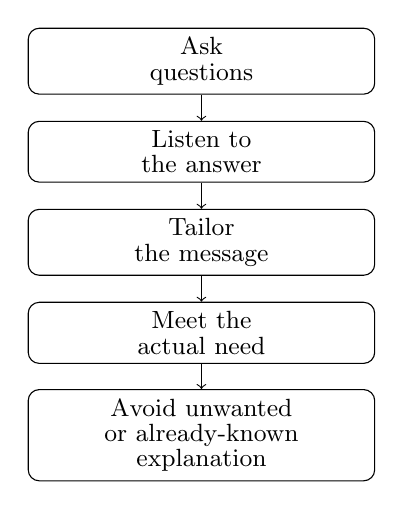
\begin{tikzpicture}[x=1cm,y=1cm]
\node[draw, rounded corners, align=center, minimum width=4.4cm, minimum height=0.72cm] (q) at (0,0) {\small Ask\\[-1mm]\small questions};
\node[draw, rounded corners, align=center, minimum width=4.4cm, minimum height=0.72cm] (l) at (0,-1.15) {\small Listen to\\[-1mm]\small the answer};
\node[draw, rounded corners, align=center, minimum width=4.4cm, minimum height=0.72cm] (t) at (0,-2.30) {\small Tailor\\[-1mm]\small the message};
\node[draw, rounded corners, align=center, minimum width=4.4cm, minimum height=0.72cm] (m) at (0,-3.45) {\small Meet the\\[-1mm]\small actual need};
\node[draw, rounded corners, align=center, minimum width=4.4cm, minimum height=0.90cm] (a) at (0,-4.75) {\small Avoid unwanted\\[-1mm]\small or already-known\\[-1mm]\small explanation};
\draw[->] (q) -- (l);
\draw[->] (l) -- (t);
\draw[->] (t) -- (m);
\draw[->] (m) -- (a);
\end{tikzpicture}
\caption{The sales process in White's account is a feedback loop, not a closing script.}
\end{figure}

A compact notation for the same idea is:
\begin{equation}
\text{Message Fit}
=
\text{Relevance to Need}
-
\text{Known or Unwanted Content}.
\end{equation}

This is conceptual notation, not a measurable formula. It says only what the interview says: the message becomes weaker when it tells people what they do not want to know, or what they already know better than the seller.

\subsection{Question \& Answer}

\paragraph{Question.}
If selling is not mainly the art of closing, what replaces it?

\paragraph{Answer.}
In White's account, the replacement is communication under feedback. We ask first, listen to the answer, and then change the message. Confidence helps, but confidence alone is not the sale. The sale becomes possible when the listener recognizes that the message has been shaped around a real need.

\section{Humility, Expertise, and Money Discipline}

White then makes the sales lesson more concrete. If he is presenting in a room of thirty people, he may ask how many medical professionals are present. When hands go up, he does not try to show that he knows health care better than they do. He says he is there to offer a vision of what he thinks could be a better system.

This is commercial humility. It is not weakness. It is the discipline of knowing what not to claim.

\begin{definition}
\emph{Commercial humility} is the operating habit of respecting what another party knows, what the business does not yet know, and what the entrepreneur has not yet earned the right to spend or claim.
\end{definition}

The next question asks for mentor advice. White begins with compression: talk too much, slow down, say what needs to be said in fewer words. The reason is practical. The speaker may know the subject well, but the listener does not yet have the same structure in mind. Excess explanation can become a burden.

Then the lesson turns to money. White says entrepreneurs must be careful about funding businesses and spending money because personal and professional life come together. He gives concrete examples: a strong week, a few thousand dollars of business, and then the temptation to buy a suit at Saks Fifth Avenue or a \(\$200\) bottle of wine.

The risk relation is:
\begin{equation}
\text{Business Win}
\longrightarrow
\text{Personal Spending Temptation}.
\end{equation}

This is not accounting. It is behavioral mechanics. A revenue event can be mistaken for durable wealth. If the owner lets that mistake govern spending, the business loses slack before it has earned stability.

White returns to humility again. He describes himself as confident and aggressive, but also as someone trying to remain aware of what he does not know. The useful entrepreneurial position is not timid ignorance and not reckless certainty. It is action with an active sense of limit:
\begin{equation}
\text{Judgment}
\approx
\text{Confidence}
+
\text{Awareness of Ignorance}.
\end{equation}

The approximation sign matters. We are not defining a law. We are preserving the balance White keeps returning to.

\section{Trauma, Brain Systems, and Claim Boundaries}

The interviewer then shifts sharply. He brings up Kanye West, the death of West's mother, mental health, medication, and relational trauma. This material belongs in the chapter because it explains the worldview behind White's company and product category. But it must remain source-conscious. What follows is White's interview claim, not independent medical advice.

White begins by broadening the word trauma. He says people often imagine trauma only as a major event with a major injury. He instead describes it as anything abnormal in day-to-day life experience. He then gives three categories:
\begin{equation}
\text{Trauma}\in
\{\text{toxic},\ \text{physical},\ \text{emotional}\}.
\end{equation}

His examples give the categories their shape. Toxic trauma includes addiction, alcohol, drugs, food sensitivity, and poisons. Physical trauma includes football injuries, falls, head impacts, traumatic brain injury, and war injuries. Emotional trauma includes loss of a loved one and betrayal.

\begin{figure}
\centering
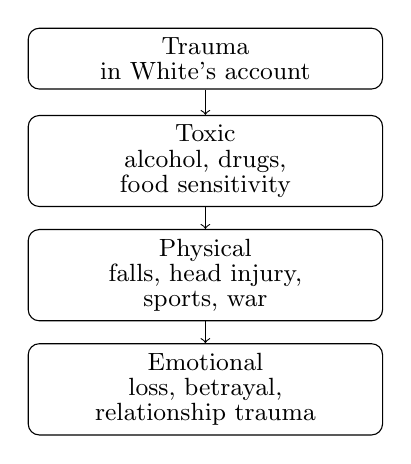
\begin{tikzpicture}[x=1cm,y=1cm]
\node[draw, rounded corners, align=center, minimum width=4.5cm, minimum height=0.75cm] (root) at (0,0) {\small Trauma\\[-1mm]\small in White's account};
\node[draw, rounded corners, align=center, minimum width=4.5cm, minimum height=0.85cm] (tox) at (0,-1.30) {\small Toxic\\[-1mm]\small alcohol, drugs,\\[-1mm]\small food sensitivity};
\node[draw, rounded corners, align=center, minimum width=4.5cm, minimum height=0.85cm] (phys) at (0,-2.75) {\small Physical\\[-1mm]\small falls, head injury,\\[-1mm]\small sports, war};
\node[draw, rounded corners, align=center, minimum width=4.5cm, minimum height=0.85cm] (emot) at (0,-4.20) {\small Emotional\\[-1mm]\small loss, betrayal,\\[-1mm]\small relationship trauma};
\draw[->] (root) -- (tox);
\draw[->] (tox) -- (phys);
\draw[->] (phys) -- (emot);
\end{tikzpicture}
\caption{A transcript-backed taxonomy of trauma. It records White's framing, not a clinical classification system.}
\end{figure}

White then introduces a two-system picture of the brain:
\begin{equation}
\text{Brain State}
\approx
(\text{Electrical System},\ \text{Chemical System}).
\end{equation}

He says the two systems do a kind of dance. Trauma, in his account, can overwhelm the protective response of the brain. Fight-or-flight may do its work in the moment, but after the trauma the system may remain disturbed. He connects that continuing disturbance to PTSD and says it is not only a military phenomenon.

The claimed manifestation channels are:
\begin{equation}
\text{Trauma Response}
\longrightarrow
\begin{cases}
\text{chemical imbalance},\\
\text{EEG or frequency pattern}.
\end{cases}
\end{equation}

White criticizes a medication-first response as, at times, a guessing game: someone feels depressed, loses desire, has trouble in marriage, and is offered a medication. The notes should not turn that into a general medical conclusion. The safer chapter-level point is that White frames his company around a systems view: trauma, health, treatment, nutrition, talk therapy, non-invasive technology, and life structure all appear in the same explanatory field.

\subsection{Question \& Answer}

\paragraph{Question.}
How does a relational trauma, such as losing a stabilizing relationship, affect the brain in White's account?

\paragraph{Answer.}
White says the loss can overwhelm the brain's protective response. In the moment, fight-or-flight may protect the person. After the event, the system may remain out of balance. In his framing, that imbalance can appear chemically, electrically, or both. The chapter should keep this as an interview claim and avoid presenting it as medical instruction.

\section{Failure as the Accomplishment}

The interviewer then pulls the conversation back to entrepreneurship: White has started companies and brought a company public, so what is the greatest accomplishment of his career? The expected answer would be an external milestone. White gives a harder answer.

His accomplishment is getting up, brushing himself off, licking his wounds, and going back in for another round. He says the worst thing after never having money is having money, losing it, and then having none. The story becomes specific: he watched his life's work loaded into trucks and taken away.

A bankruptcy attorney, Nelson Hemsley, gave him a choice. White could pay him to go to court and clean up the mess, or White could come to every meeting and courthouse appearance and face the people he owed. White describes this as a gift. The lesson was not merely legal procedure. It was consequence.

The recovery mechanism can be written as:
\begin{align}
\text{Failure}
&\longrightarrow \text{Face creditors},\\
\text{Face creditors}
&\longrightarrow \text{Return what remains},\\
\text{Return what remains}
&\longrightarrow \text{Humility},\\
\text{Humility}
&\longrightarrow \text{Renewed judgment}.
\end{align}

This is the deepest entrepreneurial turn in the interview. White does not define accomplishment as never failing. He defines it as remaining present when failure has harmed other people. He says he entered rooms where people hated him because he owed them money and they had lost money. He gave everything back, watched it divided and sold, and calls the experience brutal. On the other side, he says, he was a new man: more respectful of others, remarried to his wife, his family restored, and humility learned in a way no slogan could supply.

\subsection{Question \& Answer}

\paragraph{Question.}
Why would facing creditors count as a greater accomplishment than taking a company public?

\paragraph{Answer.}
Because in White's telling, the public-company achievement proves one kind of capability, but facing creditors proves character under consequence. It forces the entrepreneur to see the human cost of failure, return what remains, and rebuild judgment without hiding behind a representative.

\begin{remark}
The bankruptcy story should not be reduced to generic resilience. Its force is accountability. White's claimed accomplishment is not merely that he survived failure, but that he stayed present while other people bore part of the cost.
\end{remark}

\section{Structure and Small Steps}

The final movement of the interview asks about self-improvement. The interviewer frames the problem as the average modern person who is out of shape, caught in passive entertainment, and trying to get back on track. White answers with one word: structure.

He tells a story about a man named Haas, who advised him to set an alarm, get out of bed, make the bed, shower, be ready by 9 a.m., eat lunch at noon, eat dinner at six, and prepare for bed at night. The point is not that this schedule is universal. The point is that a person who has lost traction needs to be successful at something.

We can model that advice with a deliberately modest update rule. Let \(s_n\) denote self-trust after day \(n\). Let \(a_n=1\) if the person completes the one promised action for that day, and \(a_n=0\) otherwise. A qualitative reconstruction is:
\begin{equation}
s_{n+1}=s_n+\alpha a_n-\beta(1-a_n),
\qquad \alpha,\beta>0.
\end{equation}

This equation is not in the transcript. It is a compact way to express White's mechanism: completion increases self-trust, while another failed promise subtracts from it. The practical instruction is therefore to choose an action small enough that completion is likely.

\paragraph{Worked example.}
Suppose the action set for tomorrow is only
\begin{equation}
A=\{\text{set alarm},\ \text{get out of bed},\ \text{be on time}\}.
\end{equation}
Completing \(A\) does not make a person financially free. It does something more primitive: it gives evidence of follow-through. White then asks the person to sit quietly and register the fact: I did what I said I was going to do. Reflection is part of the update.

The loop is:
\begin{equation}
\text{Choose One Action}
\longrightarrow
\text{Complete It}
\longrightarrow
\text{Reflect}
\longrightarrow
\text{Repeat}.
\end{equation}

\begin{figure}
\centering
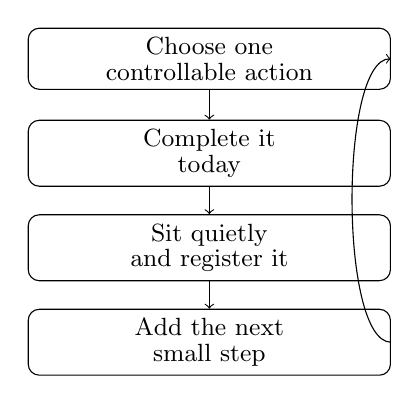
\begin{tikzpicture}[x=1cm,y=1cm]
\node[draw, rounded corners, align=center, minimum width=4.6cm, minimum height=0.75cm] (a) at (0,0) {\small Choose one\\[-1mm]\small controllable action};
\node[draw, rounded corners, align=center, minimum width=4.6cm, minimum height=0.75cm] (b) at (0,-1.20) {\small Complete it\\[-1mm]\small today};
\node[draw, rounded corners, align=center, minimum width=4.6cm, minimum height=0.75cm] (c) at (0,-2.40) {\small Sit quietly\\[-1mm]\small and register it};
\node[draw, rounded corners, align=center, minimum width=4.6cm, minimum height=0.75cm] (d) at (0,-3.60) {\small Add the next\\[-1mm]\small small step};
\draw[->] (a) -- (b);
\draw[->] (b) -- (c);
\draw[->] (c) -- (d);
\draw[->] (d.east) .. controls (1.65,-3.60) and (1.65,0) .. (a.east);
\end{tikzpicture}
\caption{The small-step loop: one completed promise becomes the evidence for attempting the next one.}
\end{figure}

\subsection{Question \& Answer}

\paragraph{Question.}
Why start with one small task instead of a total life overhaul?

\paragraph{Answer.}
Because the total overhaul creates too many failure points at once. White describes the New Year's resolution pattern: stop A, B, C, D and start E, F, G, H. The person reaches A and B, fails, feels ashamed, turns on Netflix, gets chips, and begins again from disappointment. The small task reverses the direction. It asks for one completed promise, then lets completion become proof.

The final instruction is honesty about the Achilles heel. White lists possible weak points: sugar, vodka, marijuana, a bad marriage, being mean to people. The particular examples are less important than the diagnostic rule:
\begin{equation}
\text{Useful Action}
=
\text{Small Enough to Complete}
+
\text{Close to the Real Constraint}.
\end{equation}

\section{Summary}

The interview unfolds as a sequence of practical mechanisms. First, value begins with observation: an idle car, a dinner window, a new product, and a \(\$20\) offer. Second, sales becomes a feedback loop: ask, listen, tailor, and respect what the listener already knows. Third, business income and personal spending are coupled, so a strong week is not the same as durable wealth. Fourth, White's trauma and brain-health discussion should be preserved as his claim: he frames trauma through toxic, physical, and emotional categories, and he speaks of electrical and chemical systems without giving us a clinical proof.

The final two movements carry the strongest entrepreneurial weight. Failure becomes instructive only when the entrepreneur faces the people affected by it. Self-improvement becomes durable only when it begins with one controllable promise. The chapter's mathematics is therefore the mathematics of sequences and constraints: find the service window, shape the message by feedback, protect the business from premature spending, face consequences directly, and use small completed actions to rebuild trust.